% !TEX root = ../om_ts_01.tex

\begin{frame} % frame name
	
	\videotitle{Series Components}
	
\end{frame}



\begin{frame}{Series Components: Plan}
	\begin{itemize}[<+->]
		\item Trend, cyclicity and seasonality
		\item Additive and multiplicative decomposition
		\item A formal definition?
	\end{itemize}
	
\end{frame}


\begin{frame}{Looking for components}
	
	Additive series decomposition:
	\[
	y_t = trend_t + seas_t + remainder_t
	\]
	
	\pause
	
	\alert{Trend} — smoothly changing component of the series
	
	\pause
	
	\alert{Seasonal component} — a component with a clear frequency and stable intensity
	
	\pause
	
	\alert{Random component} (remainder) — everything else
	
\end{frame}

\begin{frame}{Trend, seasonality and residual}
	
	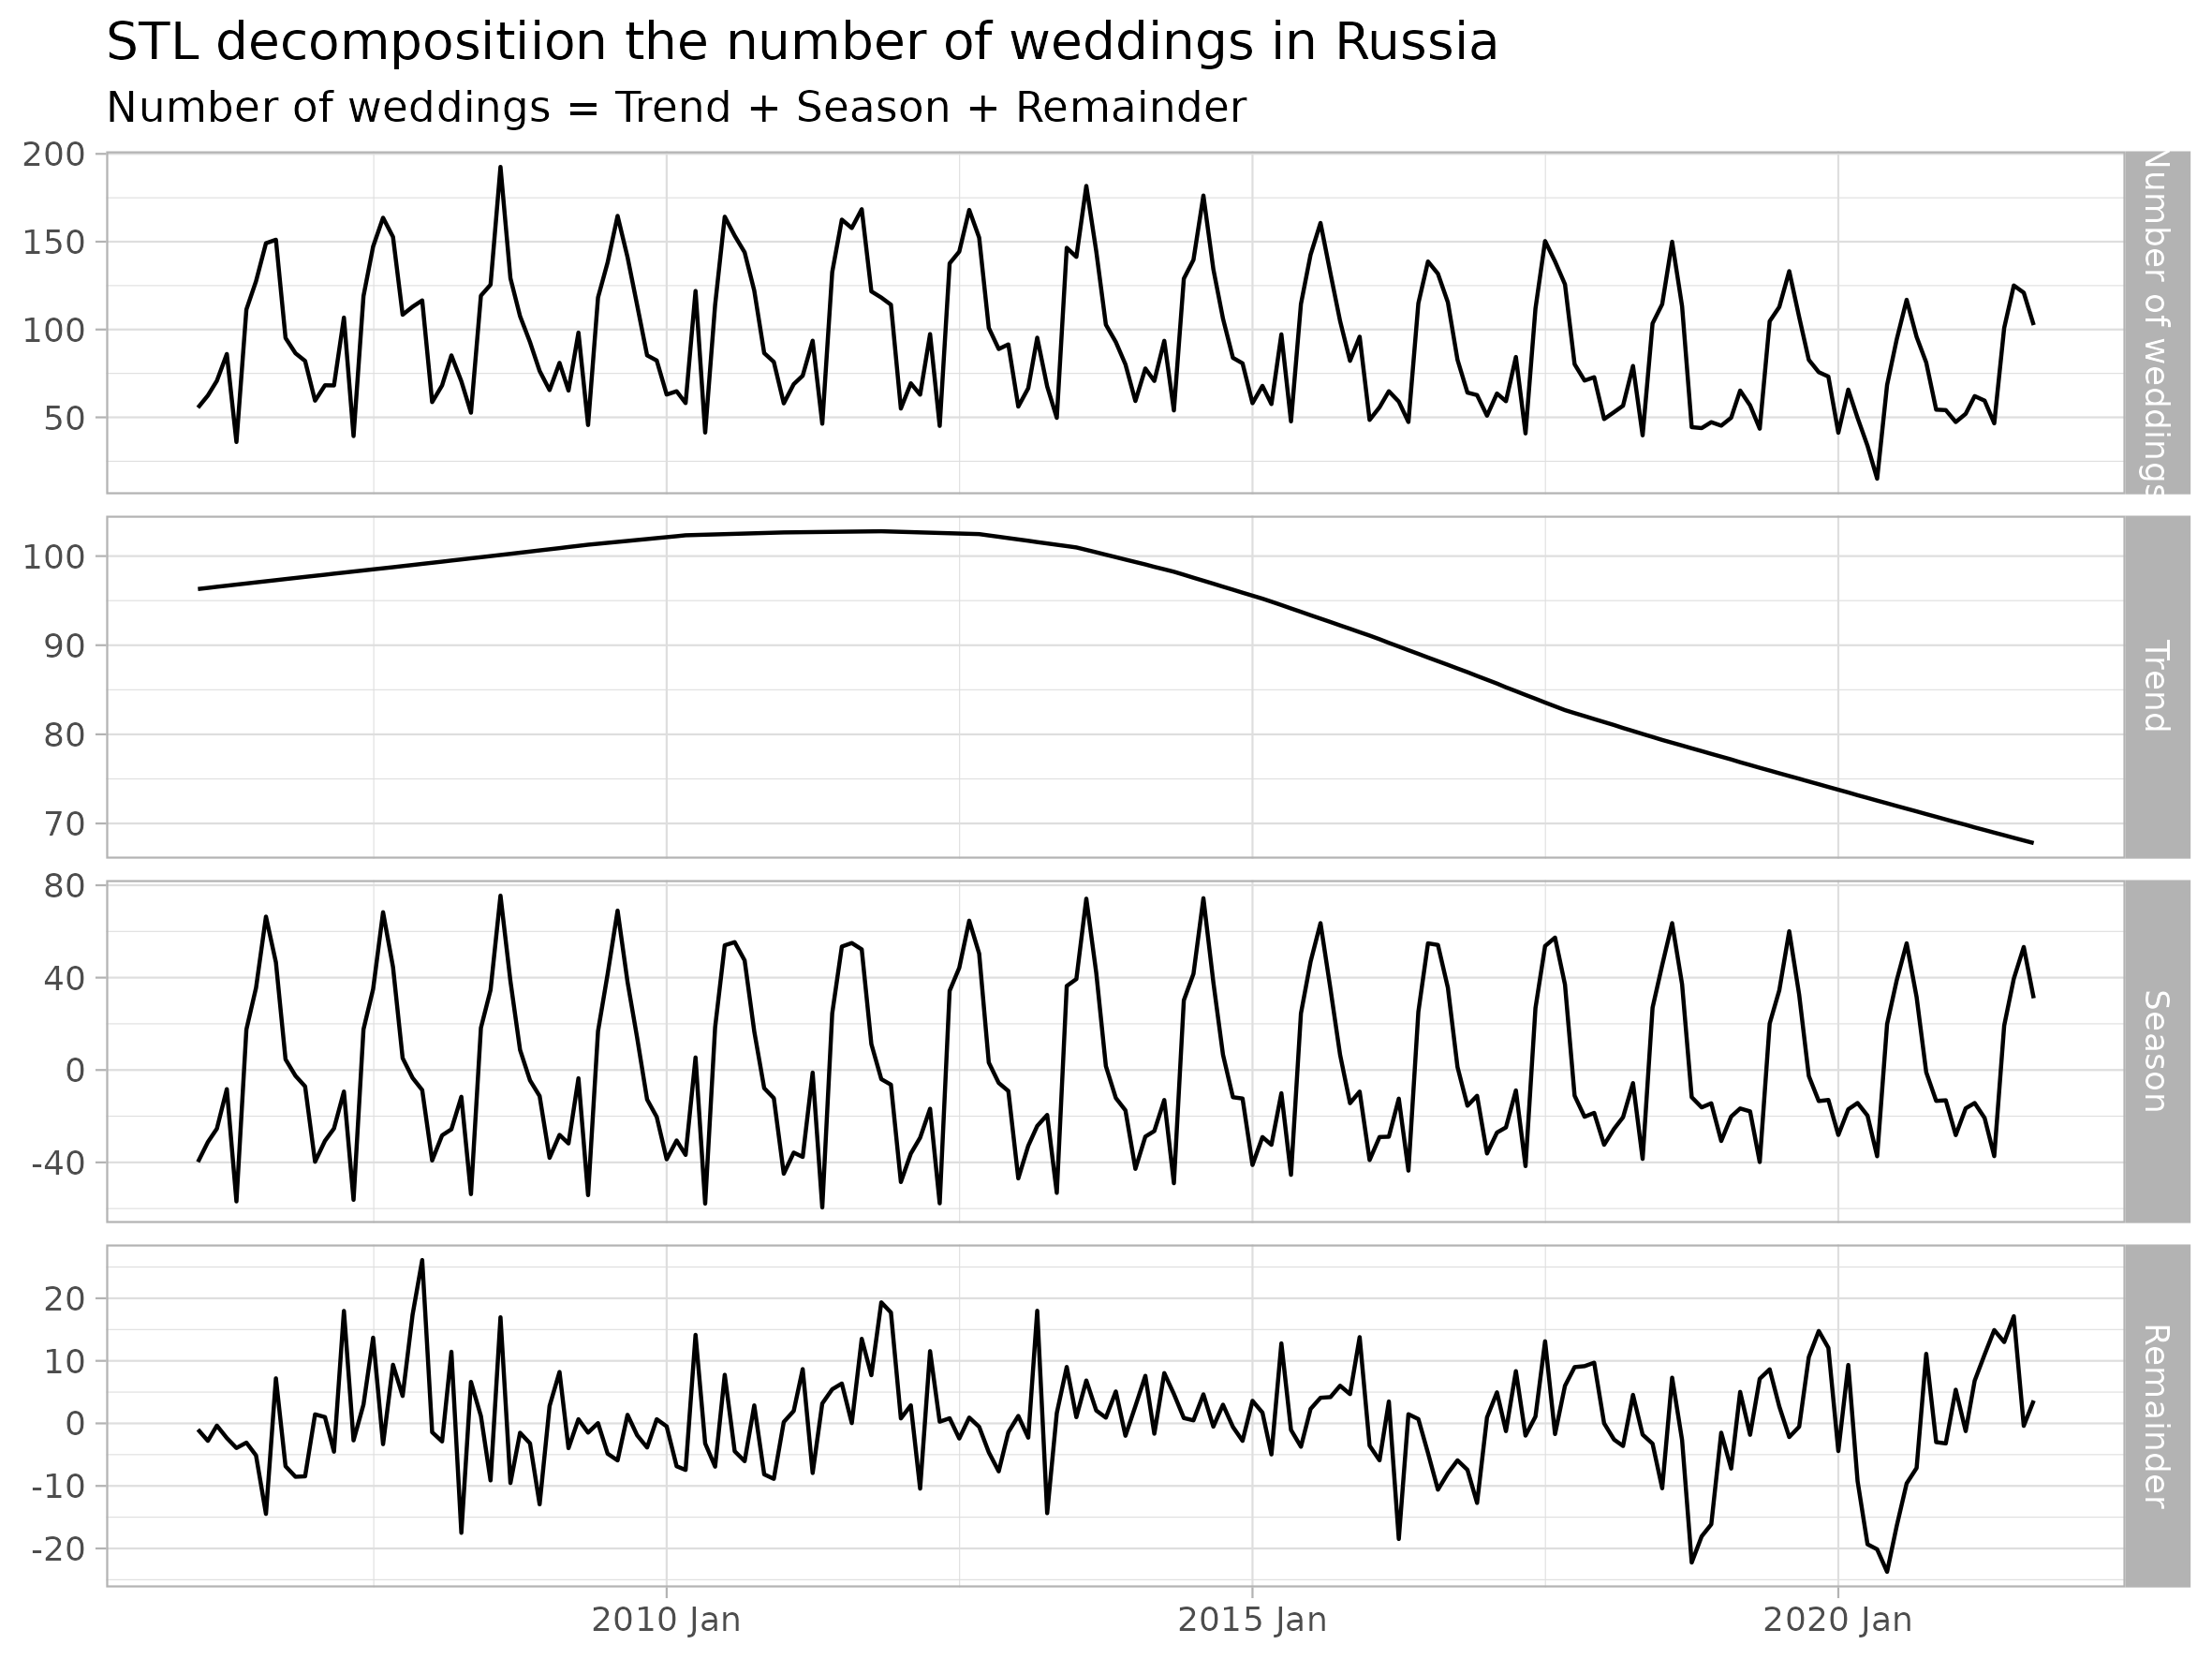
\includegraphics[width=\textwidth]{pictures/om_ts_01-041.png}
	
\end{frame}

\begin{frame}{Strict definition?}
	


	There will be no single strict definition for the components!
	
	\pause
	Some models and algorithms formally \alert{define} these components
	
\end{frame}

\begin{frame}{Cyclical component}
	
	Sometimes the series can be decomposed further
	\[
	y_t = trend_t + cycle_t + seas_t + remainder_t
	\]
	
	\pause
	\alert{Cyclical component} — component with floating frequency and unstable intensity
	
	
	\pause
	\alert{Trend} (in the narrow sense) — a smoothly changing monotonous component of a series
	
\end{frame}


\begin{frame}{Additive and multiplicative decomposition}
	
	
	\alert{Additive} series decomposition:
	\[
	y_t = trend_t + seas_t + remainder_t
	\]
	
	\pause
	\alert{Multiplicative} series decomposition:
	\[
	y_t = trend_t \cdot seas_t \cdot remainder_t
	\]
	
	\pause
	Let's transform one into another:
	\[
	\ln y_t = \ln trend_t + \ln seas_t + \ln remainder_t
	\]
\end{frame}


\begin{frame}{Box-Cox Transformation}
	
	
	For $y_t$, whose fluctuations  increases with $y_t$, \alert{it's reasonable to try} the logarithm
	or the Box-Cox transformation.
	
	\pause
	Logarithm: $y_t \to \ln y_t$
	
	Box-Cox transformation: $y_t \to bc_{\lambda}(y_t)$
	
	\pause
	
	(\alert{Generalized}) Box-Cox transformation:
	\begin{equation*}
		bc_{\lambda}(y_t) =
		\begin{cases} \ln y_t, \text{ if } \lambda = 0, \\
			\operatorname{sign} (y_t) (\abs{y_t}^{\lambda} - 1)/\lambda, \text { if } \lambda \neq 0
		\end{cases}
	\end{equation*}
	
	
	\pause
	
	How to \alert{select} the parameter $\lambda$?
	
	\pause
	
	
	\begin{itemize}[<+->]
		\item Some models contain it inside  and \alert{estimate} $\lambda$ within themselves
		\item You can choose $\lambda$ by yourself to \alert{stabilize the amplitude} of oscillations of the series
		
	\end{itemize}
	
	
\end{frame}






\begin{frame}{What to choose?}
	
	The formal definition of \alert{depends on the model}
	
	\pause
	\alert{STL algorithm}: one decomposition $y_t = trend_t + seas_t + remainder_t$
	
	\pause
	\alert{ETS(AAA)}: different decomposition $y_t = trend_t + seas_t + remainder_t$
	
	
	\pause
	It is important to understand the \alert{purpose of constructing} the decomposition
	
\end{frame}

\begin{frame}{Why decompose?}
	
	\begin{itemize}[<+->]
		\item Interesting \alert{by itself}
		\item For \alert{predicting} a series using component prediction
		\item To get \alert{characteristics of the series}
	\end{itemize}
	
	\pause
	Why characteristics?
	
	\begin{itemize}[<+->]
		\item To classify the new series into one of the given classes
		\item To identify unknown clusters in series
	\end{itemize}
	
\end{frame}


\begin{frame}{Series Components: Summary}
	\begin{itemize}[<+->]
		\item Trend \alert{smoothly changes} and includes a cyclical component
		\item The seasonal component has \alert{clear periodicity} and \alert{stable amplitude}
		\item The exact formalization of the components \alert{depends on the model}
	\end{itemize}
	
\end{frame}